\section{Auswertung}
\label{sec:Auswertung}
Am Ausgang Osc. varieeren die Spannungsamplituden; Ref. leifert eine konstante Spannung, welche \SI {22,8}{\volt} beträgt.

\subsection{Ohne Rauschen}
Ein sinusförmiges Signal mit $U = \SI{10}{\milli \volt}$ und $f = \SI{1}{\kilo \Hz}$ wird mit einem ebenfalls sinusförmigen Referenzsignal gleicher Frequenz gemischt. Das Ausgangssignal soll für fünf Phasenverschiebungen abgebildet werden, sowie das Signal nach Integration durch den Tiefpass.

\begin{figure}
  \centering
  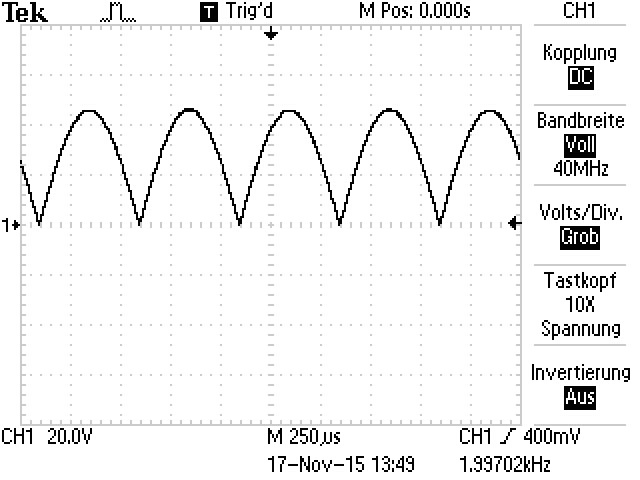
\includegraphics[width=\textwidth]{bilder/Ohne Rauschen/1.JPG}
  \caption{Phasenverschiebung 0°}.
  \label{fig:bild1}
\end{figure}

\begin{figure}
  \centering
  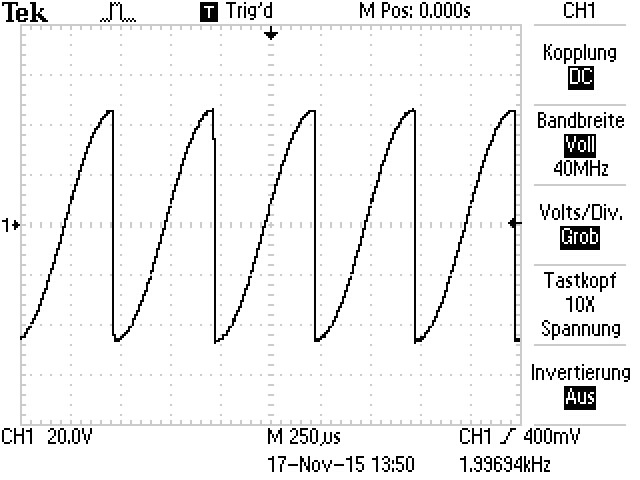
\includegraphics[width=\textwidth]{bilder/Ohne Rauschen/2.JPG}
  \caption{Phasenverschiebung 90°}.
  \label{fig:bild2}
\end{figure}

\begin{figure}
  \centering
  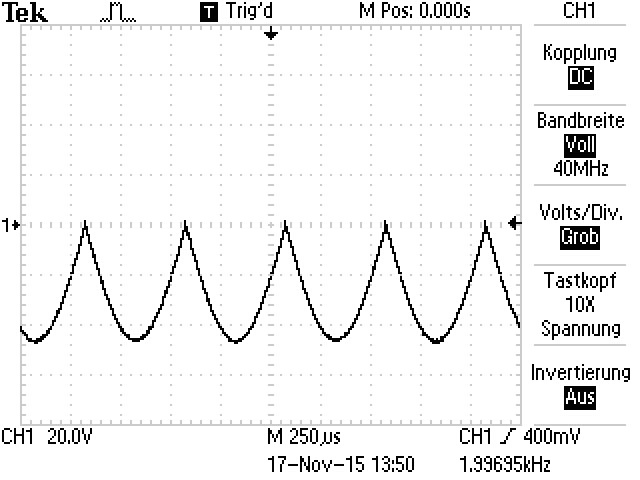
\includegraphics[width=\textwidth]{bilder/Ohne Rauschen/3.JPG}
  \caption{Phasenverschiebung 180°}.
  \label{fig:bild3}
\end{figure}

\begin{figure}
  \centering
  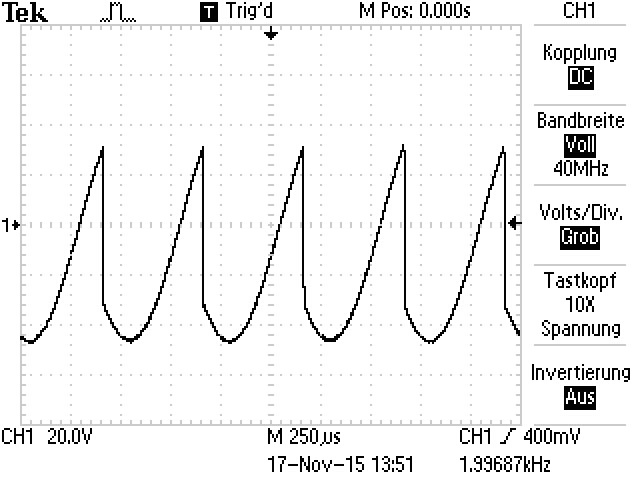
\includegraphics[width=\textwidth]{bilder/Ohne Rauschen/4.JPG}
  \caption{Phasenverschiebung 225°}.
  \label{fig:bild4}
\end{figure}

\begin{figure}
  \centering
  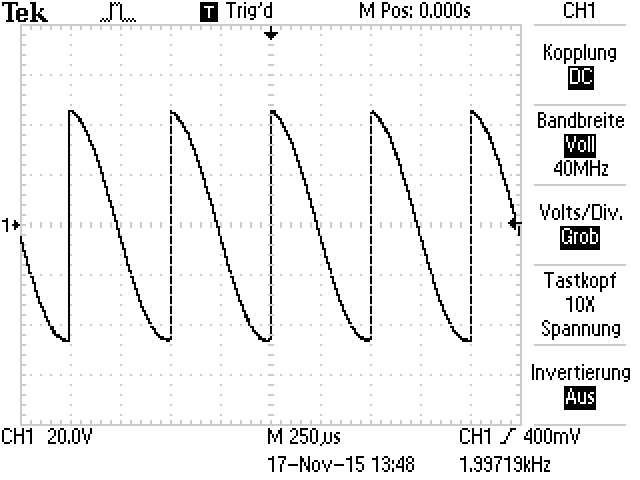
\includegraphics[width=\textwidth]{bilder/Ohne Rauschen/5.JPG}
  \caption{Phasenverschiebung 270°}.
  \label{fig:bild5}
\end{figure}

\begin{figure}
  \centering
  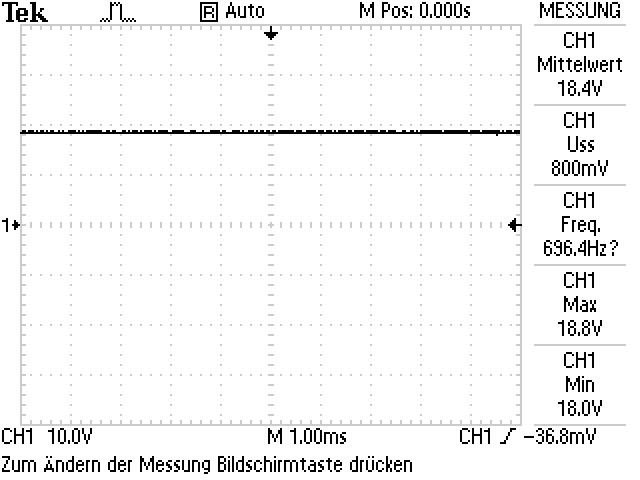
\includegraphics[width=\textwidth]{bilder/Ohne Rauschen/6.JPG}
  \caption{Signal nach Integratopn durch den Tiefpass}.
  \label{fig:bild6}
\end{figure}

Wird die Ausgangsspannung in Abhängigkeit von der Phasenverschiebung gemessen, ergeben sich folgende Messwerte.

\begin{table}
  \centering
  \caption{Ausgangsspannung ohne Rauschen}
  \label{tab:ohne_Rauschen}
  \begin{tabular}{cc}
    \toprule {$\phi \:/\: °$} & {$U \:/\: \si{\volt}$} \\
    \midrule
     0  & 32.9  \\
     15  & 32.1  \\
     30 & 28.4 \\
     45 & 20.8 \\
     60 & 9.37 \\
     75 & 0.728\\
     90 & -3.00 \\
     105 & -7.35  \\
     120 & -16.4 \\
     135 & -26.1 \\
     150 & -31.9  \\
     165 & -33.40 \\
     180 & -33.4  \\
     195 & -32.7  \\
     210 & -29.6  \\
     225 & -21.8  \\
     240 & -10.8\\
     255 & -1.26  \\
     270 & 2.52  \\
     285 & 7.22  \\
     300 & 16.0 \\
     315 & 25.7 \\
     330 & 33.1 \\
     345 & 33.1 \\
\bottomrule
\end{tabular}
\end{table}

Die gemessenen Werte sollen mit GLEICHUNG... verglichen werden.


\begin{figure}[htpb]
  \centering
  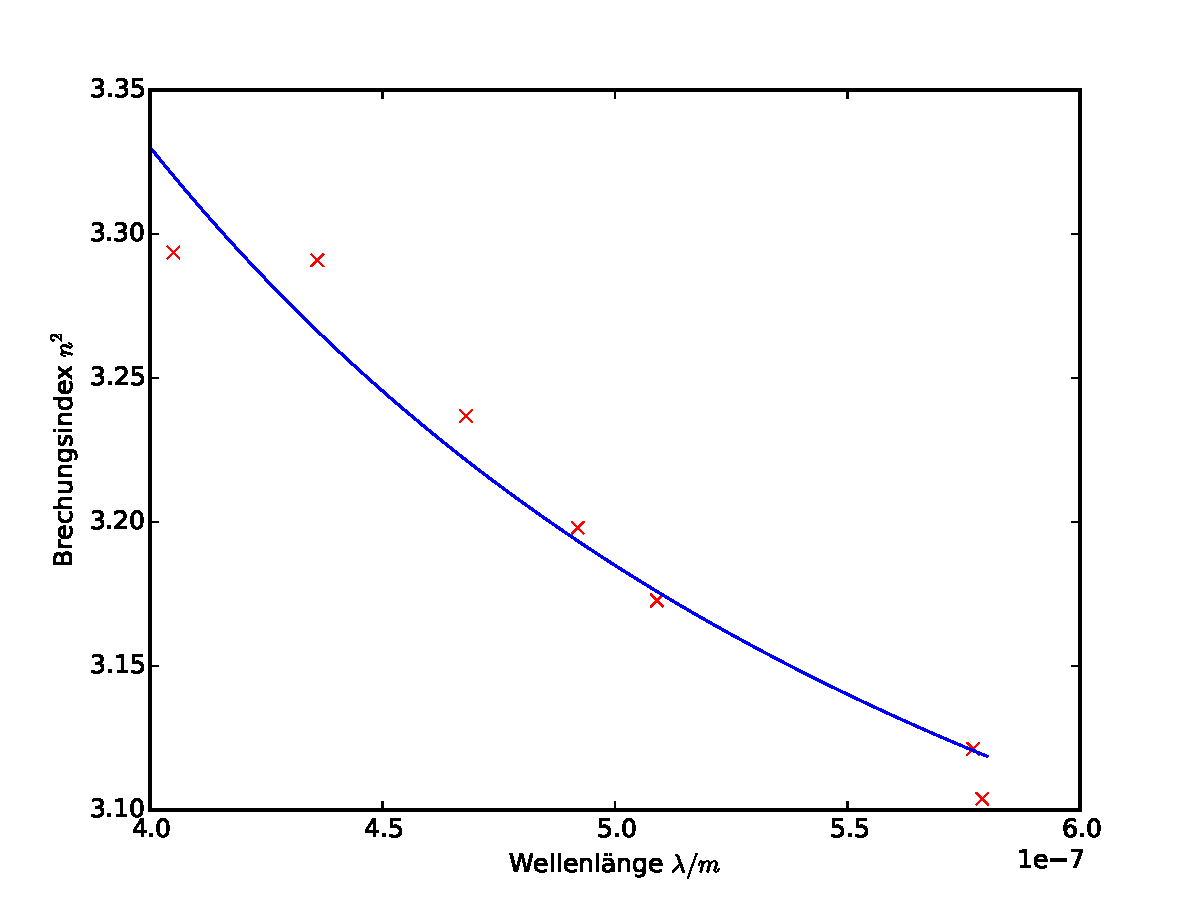
\includegraphics{plot.pdf}
  \caption{Plot der Messwerte im Vergleich mit der Ausgangaangsspannung nach der Formel $U_{\mathrm{out}} = \frac{2}{pi}U_0 \cos(\phi)$ (mit $U_0 = \SI{22,8}{\volt}$)
  \label{fig:}
\end{figure}
 Die Graphen unterscheiden sich lediglich in ihrer Amplitude.Die Amplitude des Graphen der Messwerte ist doppelt so groß wie die des Graphen, der sich aus GLEICHUNG... ergibt.

 \subsection {Mit Rauschen}
 Unter Hinzufügen eines Rauschsignals sollen erneut fünf Phasen abgebildet werden.

 \begin{figure}
   \centering
   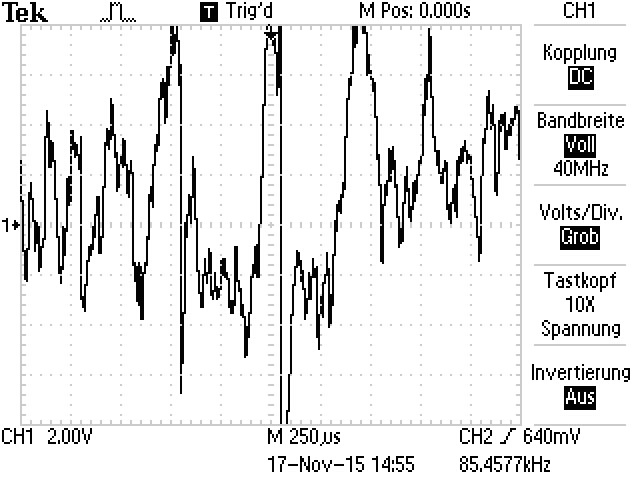
\includegraphics[width=\textwidth]{bilder/Mit Rauschen/1.JPG}
 \caption{Phasenverschiebung 0°}.
   \label{fig:1}
 \end{figure}

 \begin{figure}
   \centering
   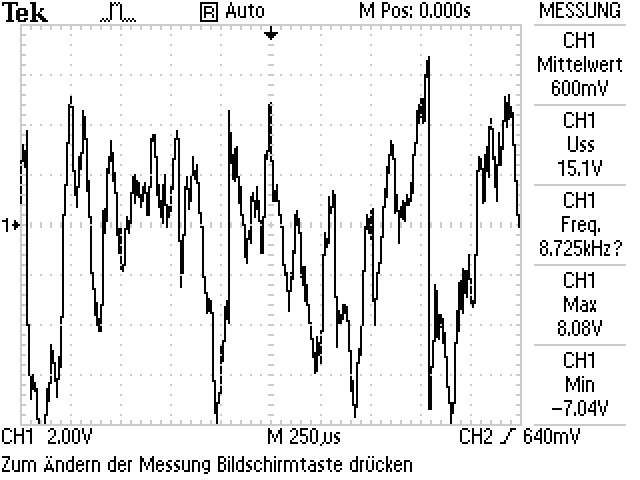
\includegraphics[width=\textwidth]{bilder/Mit Rauschen/2.JPG}
 \caption{Phasenverschiebung 90°}.
   \label{fig:2}
 \end{figure}

 \begin{figure}
   \centering
   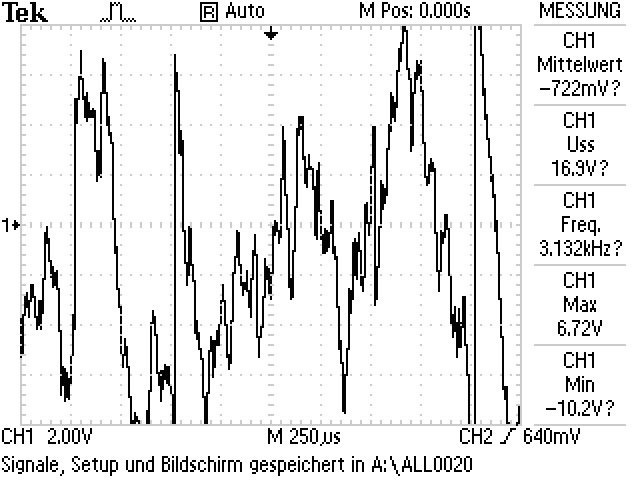
\includegraphics[width=\textwidth]{bilder/Mit Rauschen/3.JPG}
 \caption{Phasenverschiebung 180°}.
   \label{fig:3}
 \end{figure}

 \begin{figure}
   \centering
   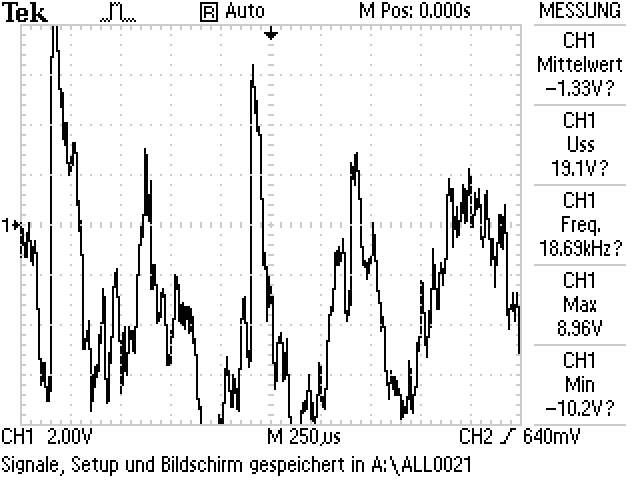
\includegraphics[width=\textwidth]{bilder/Mit Rauschen/4.JPG}
 \caption{Phasenverschiebung 225°}.
   \label{fig:4}
 \end{figure}

 \begin{figure}
   \centering
   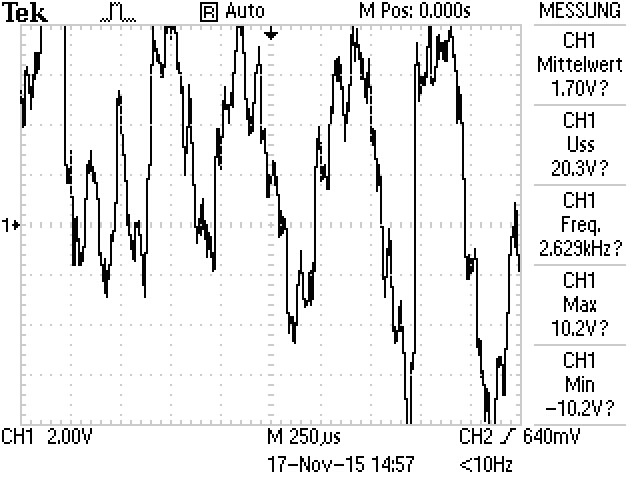
\includegraphics[width=\textwidth]{bilder/Mit Rauschen/5.JPG}
 \caption{Phasenverschiebung 270°}.
   \label{fig:5}
 \end{figure}

 \begin{figure}
   \centering
   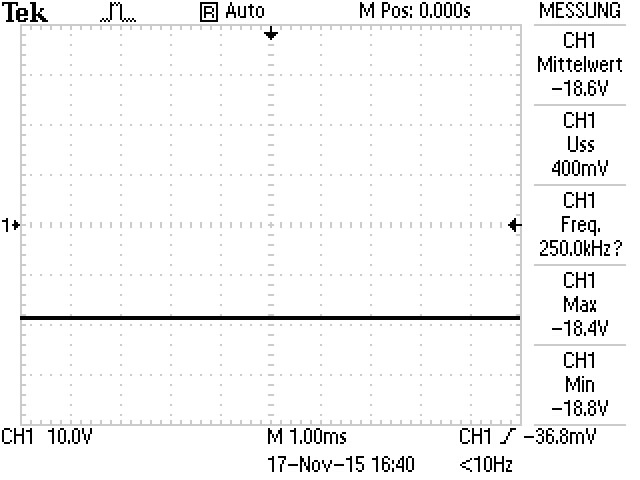
\includegraphics[width=\textwidth]{bilder/Mit Rauschen/6.JPG}
 \caption{Signal nach Integration durch den Tiefpass}.
   \label{fig:6}
 \end{figure}

Für die Ausgangsspannung in Abhängigkeit von der Phasenverschiebung ergeben sich folgende Messwerte.
\begin{table}
  \centering
  \caption{Ausgangsspannung mit Rauschen}
  \label{tab:ohne_Rauschen}
  \begin{tabular}{cc}
    \toprule {$\phi \:/\: °$} & {$U \:/\: \si{\volt}$} \\
    \midrule
    0	& 33.0 \\
    15 & 31.7 \\
    30 & 28.0 \\
    45	& 21.5 \\
    60 & 9.28 \\
    75 & 0.1 \\
    90	& -3.31 \\
    105 & -7.91 \\
    120	& -16.1 \\
    135	& -24.8 \\
    150	& -31.3 \\
    165 & -33.0 \\
    180	& -33.5 \\
    195	& -31.2 \\
    210	& -28.1 \\
    225	& -21.8 \\
    240 & -9.56 \\
    255	& -2.01 \\
    270	& 2.95 \\
    285	& 7.80 \\
    300	& 15.3 \\
    315	& 25.7 \\
    330	& 30.8 \\
    345	& 32.8 \\
    \bottomrule
    \end{tabular}
\end{table}

\subsection{Photodetektorschaltung}
Bei ausgeschalteter LED beträgt die Spannung$U_{\mathrm{null} = \SI {-7,72}{\volt}}$.
Die Blinkfrequenz wird auf $f = \SI {321,3}{\Hz}$ und der Low-Pass-Amplifier auf Gain 1000 eingestellt.

\begin{table}
  \centering
  \caption{Photodetektorspannung $U_{\mathrm{out}}}$ in Abhängigkeit des Abstandes $r$
  \label{tab:photodetektor}
  \begin{tabular}{cc}
    \toprule {$r \:/\: meter$} & {$U_{\mathrm{out}} \:/\: \si{\volt}$} \\
    \midrule
     0.1 & 88.2 \\
     0.15 & 28.6 \\
     0.2 & 11.0 \\
     0.25 & 3.61 \\
     0.3 & -0.165 \\
     0.35 & -2.00 \\
     0.4 & -3.53 \\
     0.45 & -4.45 \\
     0.5 & -5.05 \\
     0.55 & -5.43 \\
     0.6 & -5.76 \\
     0.65 & -6.08 \\
     0.7 & -6.31 \\
     0.75 & -6.45 \\
     0.8 & -6.61 \\
     0.85 & -6.72 \\
     0.9 & -6.80 \\
     0.95 & -6.84 \\
     1 & -6.95 \\
     1.05 & -7.01 \\
     1.1 & -7.04 \\
     1.15 & -7.08 \\
     1.2 & -7.11 \\
     1.25 & -7.14 \\
     1.3 & -7.18 \\
     1.35 & -7.21 \\
     1.4 & -7.24 \\
     1.45 & -7.27 \\
     1.5 & -7.30 \\
     1.55 & -7.34 \\
     1.6 & -7.35 \\
     1.65 & -7.37 \\
     1.7 & -7.39 \\
     1.75 & -7.43 \\
     1.8 & -7.44 \\
     1.85 & -7.43 \\
     1.9 & -7.43 \\
     \bottomrule
    \end{tabular}
   \end{table}

Die bereinigten Messwerte ergeben sich aus
\begin{equation}
  U_{\mathrm{ber}} = \frac{U_{\mathrm{out}}}{\text{Gain}} - {U_{\mathrm{null}}}{1000}
\end {equation}
